
\documentclass[a4paper,12pt,twoside]{article}
\usepackage{xcolor}
\definecolor{verde}{rgb}{0,0.5,0}
\definecolor{jpurple}{rgb}{0.5,0,0.35}
\usepackage[utf8]{inputenc}
\usepackage{graphicx}
\usepackage{float}
\usepackage[brazilian]{babel}
\usepackage{indentfirst}
\usepackage{steinmetz}
\usepackage{multicol}
\usepackage[left=2cm, right=2cm, top=2cm]{geometry}
\setlength\parindent{1cm}
\usepackage{mathrsfs, amsmath}
\usepackage{textcomp}
\usepackage{gensymb}
\usepackage{lipsum}
\usepackage{natbib}
\usepackage{listings}
\lstset{
  language=vhdl,
  basicstyle=\ttfamily\small, 
  keywordstyle=\color{blue}, 
  stringstyle=\color{verde}, 
  commentstyle=\color{red}, 
  extendedchars=true, 
  showspaces=false, 
  showstringspaces=false, 
  numbers=left,
  numberstyle=\tiny,
  breaklines=true, 
  backgroundcolor=\color{jpurple!10},
  breakautoindent=true, 
  captionpos=b,
  xleftmargin=0pt,
}

\headheight = 10pt

\setcounter{section}{-1}



\date{}

\begin{document}

\begin{titlepage}
\begin{center}
{\large Universidade Federal do Rio de Janeiro}\\[0.2cm]
{\large Engenharia Eletrônica e de Computação}\\[0.2cm]
{\large Trabalho de Sistemas Digitais}\\[5.1cm]
{\bf \huge FORCA - 2° Trabalho}\\[5.1cm]
\end{center}
{\large Alunos(as): Gabriel de Lima Moura e Karen dos Anjos Arcoverde}\\[0.7cm]
{\large Professor: Luís Henrique Maciel Kosmalski Costa}\\[5.1cm]
\begin{center}
{\large Rio de Janeiro}\\[0.2cm]
{\large 2019.2}
\end{center}
\end{titlepage}

\renewcommand{\contentsname}{Sumário}

\tableofcontents
\clearpage
%%%%%%%%%%%%%%%%%%%%%%%%%%%%%%%%%%%%%%%%%%%%%%%%%%%%%%%%%%%%%%%%%%%
\section{Introdução}
Este trabalho tem como objetivo o desenvolvimento de um "Jogo da Forca".
O projeto foi feito utilizando o Kit Xilinx Spartan3 e um teclado conecatdo à placa FPGA através de um cabo ps2. Para isso, foram utilizados 4 módulos previamente desenvolvidos para o funcionamento do teclado e do visor LCD:
 \begin{itemize}
   \item ps2\_rx.vhdl
   \item fifo.vhdl
   \item kb\_lcode.vhdl
   \item key2ascii.vhdl
 \end{itemize}
 
 As conexões dos 4 módulos podem ser esquematizados em um diagrama:
 \begin{figure}[H]
\centering
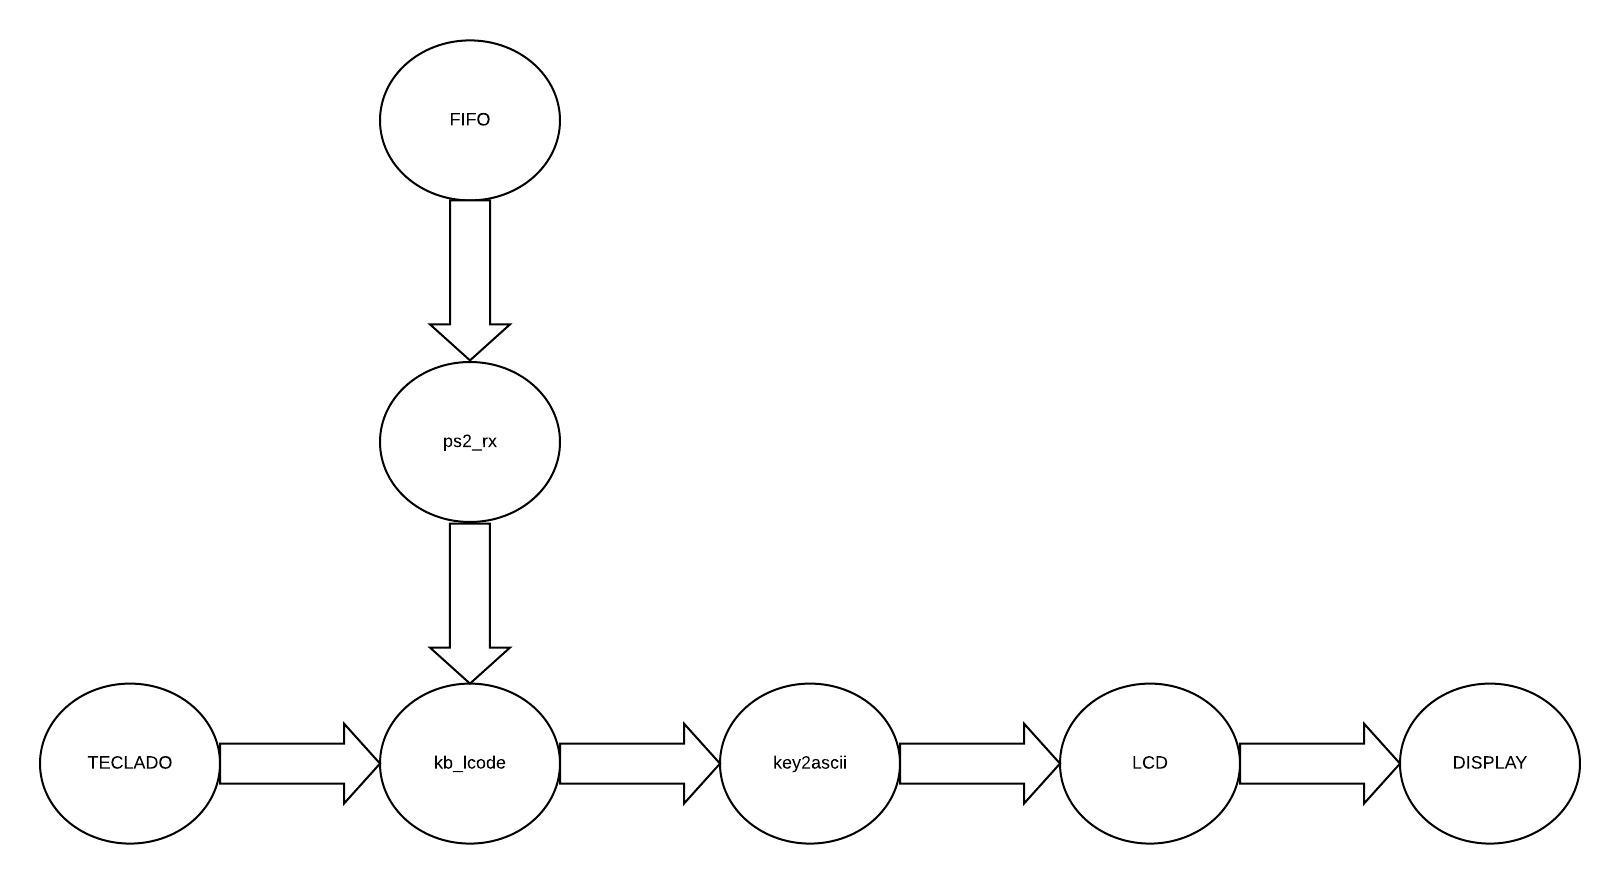
\includegraphics[scale=0.6]{diagramadeblocos.jpeg}
\caption{Diagrama de blocos dos módulos}
\label{fig:diagrama}
\end{figure}
 
    
Para o projeto foi planejada uma máquina de estados que serviu de base para o desenvolvimento da lógica do jogo.
%%%%%%%%%%%%%%%%%%%%%%%%%%%%%%%%%%%%%%%%%%%%%%%%%%%%%%%%%%
\section{Desenvolvimento}

%%%%%%%%%%%%%%%%% PS2.VHD
\subsection{PS2}
O módulo ps2-rx realiza o contato direto com o teclado fazendo retornos de 8 bits para as teclas pressionadas. O conector ps2 é um conector mini-DIN de 6 pinos usado para conectar teclados e mouses a um sistema computacional (Figura \ref{fig:ps2-conector}). 

\begin{figure}[H]
\centering
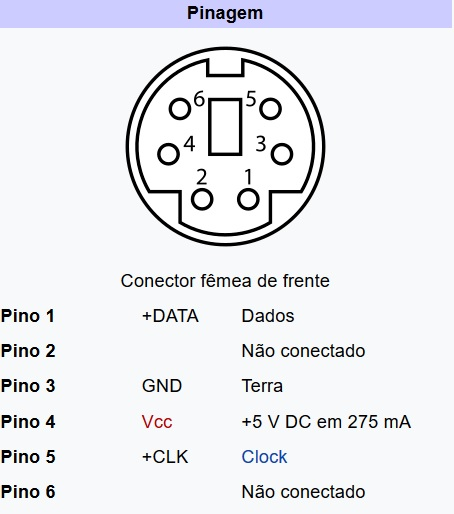
\includegraphics[scale=0.8]{ps2.jpg}
\caption{conector ps2}
\label{fig:ps2-conector}
\end{figure}

Para a comunicação com o teclado, as entradas ps2d e ps2c são passadas para o programa representando os pinos 1 e 5 respectivamente. O código não foi alterado.

\begin{figure}[H]
\centering
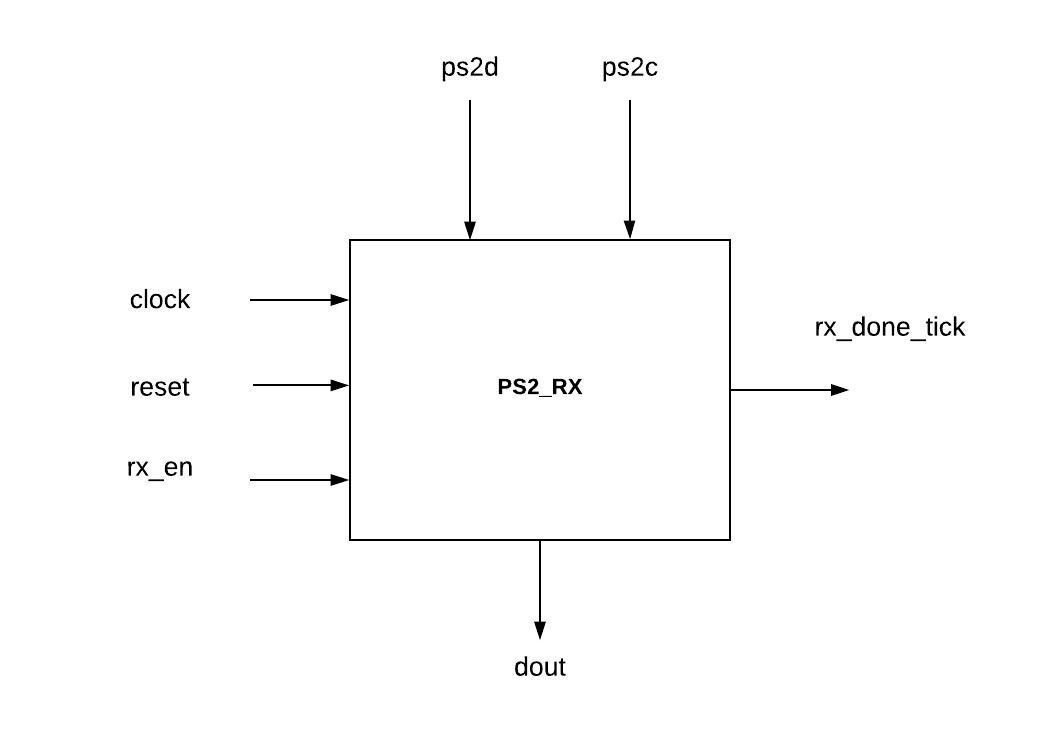
\includegraphics[scale=0.8]{ps2rx.jpeg}
\caption{Módulo ps2-rx}
\label{fig:ps2rx}
\end{figure}


\begin{lstlisting}
-- Listing 8.1
library ieee;
use ieee.std_logic_1164.all;
use ieee.numeric_std.all;
entity ps2_rx is
   port (
      clk, reset: in  std_logic;
      ps2d, ps2c: in  std_logic;  -- key data, key clock
      rx_en: in std_logic;
      rx_done_tick: out  std_logic;
      dout: out std_logic_vector(7 downto 0)
   );
end ps2_rx;

architecture arch of ps2_rx is
   type statetype is (idle, dps, load);
   signal state_reg, state_next: statetype;
   signal filter_reg, filter_next:
          std_logic_vector(7 downto 0);
   signal f_ps2c_reg,f_ps2c_next: std_logic;
   signal b_reg, b_next: std_logic_vector(10 downto 0);
   signal n_reg,n_next: unsigned(3 downto 0);
   signal fall_edge: std_logic;
begin
   --=================================================
   -- filter and falling edge tick generation for ps2c
   --=================================================
   process (clk, reset)
   begin
      if reset='1' then
         filter_reg <= (others=>'0');
         f_ps2c_reg <= '0';
      elsif (clk'event and clk='1') then
         filter_reg <= filter_next;
         f_ps2c_reg <= f_ps2c_next;
      end if;
   end process;

   filter_next <= ps2c & filter_reg(7 downto 1);
   f_ps2c_next <= '1' when filter_reg="11111111" else
                  '0' when filter_reg="00000000" else
                  f_ps2c_reg;
   fall_edge <= f_ps2c_reg and (not f_ps2c_next);

   --=================================================
   -- fsmd to extract the 8-bit data
   --=================================================
   -- registers
   process (clk, reset)
   begin
      if reset='1' then
         state_reg <= idle;
         n_reg  <= (others=>'0');
         b_reg <= (others=>'0');
      elsif (clk'event and clk='1') then
         state_reg <= state_next;
         n_reg <= n_next;
         b_reg <= b_next;
      end if;
   end process;
   -- next-state logic
   process(state_reg,n_reg,b_reg,fall_edge,rx_en,ps2d)
   begin
      rx_done_tick <='0';
      state_next <= state_reg;
      n_next <= n_reg;
      b_next <= b_reg;
      case state_reg is
         when idle =>
            if fall_edge='1' and rx_en='1' then
               -- shift in start bit
               b_next <= ps2d & b_reg(10 downto 1);
               n_next <= "1001";
               state_next <= dps;
            end if;
         when dps =>  -- 8 data + 1 pairty + 1 stop
            if fall_edge='1' then
            b_next <= ps2d & b_reg(10 downto 1);
               if n_reg = 0 then
                   state_next <=load;
               else
                   n_next <= n_reg - 1;
               end if;
            end if;
         when load =>
            -- 1 extra clock to complete the last shift
            state_next <= idle;
            rx_done_tick <='1';
      end case;
   end process;
   -- output
   dout <= b_reg(8 downto 1); -- data bits
end arch;
} \end{lstlisting}

%%%%%%%%%%%%%%%%% FIFO.vhd
\subsection{FIFO}
O módulo fifo.vhdl representa uma estrutura de dados utilizada para armazenar os vetores de 8 bits que indicam a tecla lida. A estrutura do tipo Fifo (first in first out) é caracterizada por um algoritmo onde o primeiro elemento a ser retirado é o primeiro que tiver sido inserido (Figura \ref{fig:fifo}). 

\begin{figure}[H]
\centering
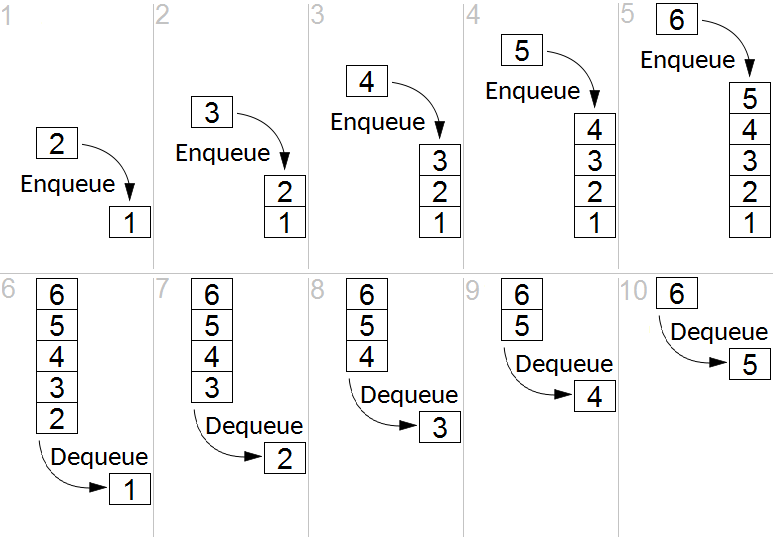
\includegraphics[scale=0.7]{Fifo_queue.png}
\caption{representação de uma fifo}
\label{fig:fifo}
\end{figure}

A FIFO previamente desenvolvida possuía 4 bits de espaço, o que poderia gerar um atraso de 4 teclas à cada leitura. Porém, esse problema foi contornado pela lógica do jogo e o código da fifo não precisou ser alterado.

\begin{figure}[H]
\centering
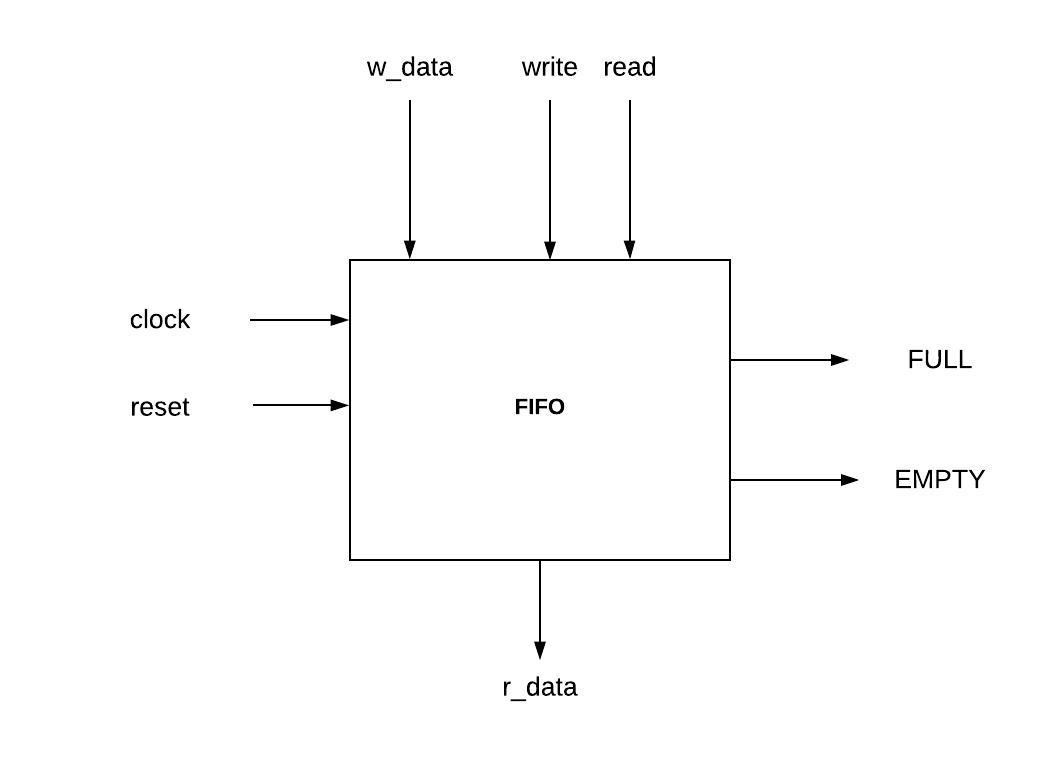
\includegraphics[scale=0.7]{fifo.jpeg}
\caption{Módulo FIFO}
\label{fig:modulofifo}
\end{figure}



\begin{lstlisting}
-- Listing 4.20
library ieee;
use ieee.std_logic_1164.all;
use ieee.numeric_std.all;
entity fifo is
   generic(
      B: natural:=8; -- number of bits
      W: natural:=4 -- number of address bits
   );
   port(
      clk, reset: in std_logic;
      rd, wr: in std_logic;
      w_data: in std_logic_vector (B-1 downto 0);
      empty, full: out std_logic;
      r_data: out std_logic_vector (B-1 downto 0)
   );
end fifo;

architecture arch of fifo is
   type reg_file_type is array (2**W-1 downto 0) of
        std_logic_vector(B-1 downto 0);
   signal array_reg: reg_file_type;
   signal w_ptr_reg, w_ptr_next, w_ptr_succ:
      std_logic_vector(W-1 downto 0);
   signal r_ptr_reg, r_ptr_next, r_ptr_succ:
      std_logic_vector(W-1 downto 0);
   signal full_reg, empty_reg, full_next, empty_next:
          std_logic;
   signal wr_op: std_logic_vector(1 downto 0);
   signal wr_en: std_logic;
begin
   --=================================================
   -- register file
   --=================================================
   process(clk,reset)
   begin
     if (reset='1') then
        array_reg <= (others=>(others=>'0'));
     elsif (clk'event and clk='1') then
        if wr_en='1' then
           array_reg(to_integer(unsigned(w_ptr_reg)))
                 <= w_data;
        end if;
     end if;
   end process;
   -- read port
   r_data <= array_reg(to_integer(unsigned(r_ptr_reg)));
   -- write enabled only when FIFO is not full
   wr_en <= wr and (not full_reg);

   --=================================================
   -- fifo control logic
   --=================================================
   -- register for read and write pointers
   process(clk,reset)
   begin
      if (reset='1') then
         w_ptr_reg <= (others=>'0');
         r_ptr_reg <= (others=>'0');
         full_reg <= '0';
         empty_reg <= '1';
      elsif (clk'event and clk='1') then
         w_ptr_reg <= w_ptr_next;
         r_ptr_reg <= r_ptr_next;
         full_reg <= full_next;
         empty_reg <= empty_next;
      end if;
   end process;

   -- successive pointer values
   w_ptr_succ <= std_logic_vector(unsigned(w_ptr_reg)+1);
   r_ptr_succ <= std_logic_vector(unsigned(r_ptr_reg)+1);

   -- next-state logic for read and write pointers
   wr_op <= wr & rd;
   process(w_ptr_reg,w_ptr_succ,r_ptr_reg,r_ptr_succ,wr_op,
           empty_reg,full_reg)
   begin
      w_ptr_next <= w_ptr_reg;
      r_ptr_next <= r_ptr_reg;
      full_next <= full_reg;
      empty_next <= empty_reg;
      case wr_op is
         when "00" => -- no op
         when "01" => -- read
            if (empty_reg /= '1') then -- not empty
               r_ptr_next <= r_ptr_succ;
               full_next <= '0';
               if (r_ptr_succ=w_ptr_reg) then
                  empty_next <='1';
               end if;
            end if;
         when "10" => -- write
            if (full_reg /= '1') then -- not full
               w_ptr_next <= w_ptr_succ;
               empty_next <= '0';
               if (w_ptr_succ=r_ptr_reg) then
                  full_next <='1';
               end if;
            end if;
         when others => -- write/read;
            w_ptr_next <= w_ptr_succ;
            r_ptr_next <= r_ptr_succ;
      end case;
   end process;
   -- output
   full <= full_reg;
   empty <= empty_reg;
end arch;
} \end{lstlisting}


%%%%%%%%%%%%%%%%% Kb_code.vhd
\subsection{kbcode}
O módulo kbcode foi utilizado para a leitura das teclas pressionadas no teclado e armazenamento desses dados na fifo. Para isso, ele faz uso dos módulos fifo.vhdl e ps2\_rx.vhdl previamente analisados. O código não precisou ser alterado. 


\begin{figure}[H]
\centering
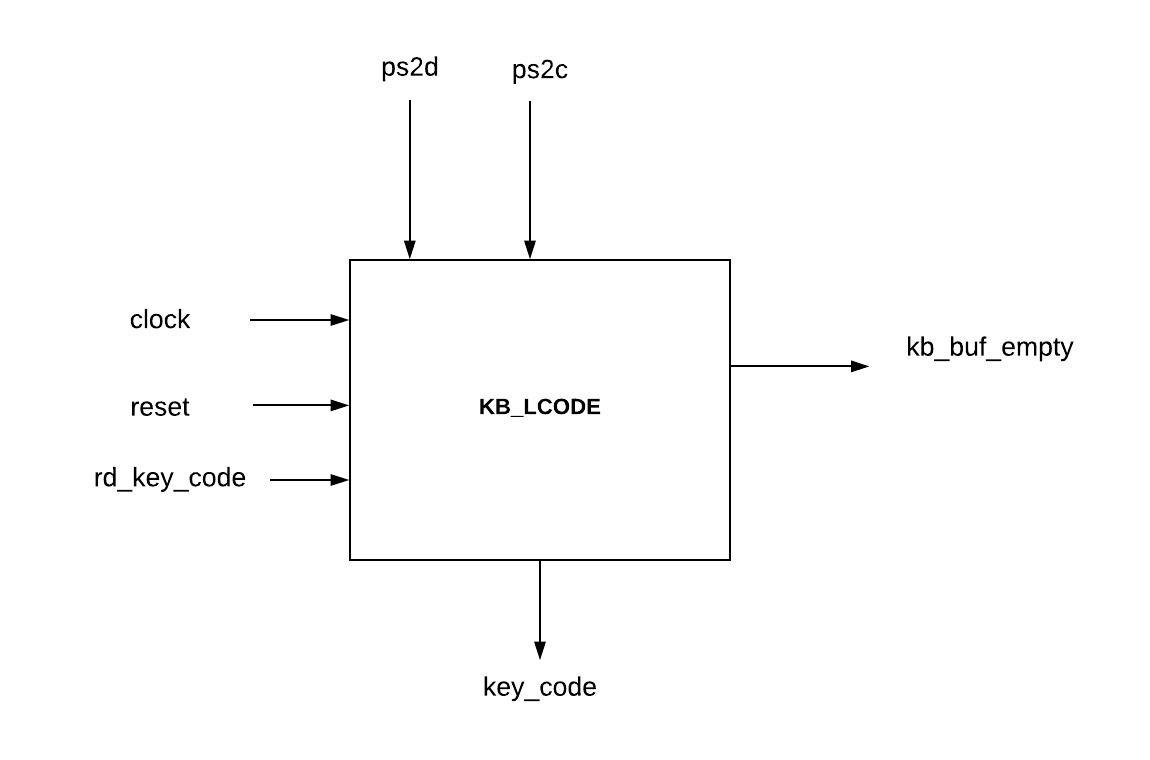
\includegraphics[scale=0.6]{kblcode.jpeg}
\caption{Módulo kbl-code}
\label{fig:kblcode}
\end{figure}

\begin{lstlisting}
-- Listing 8.3
library ieee;
use ieee.std_logic_1164.all;
use ieee.numeric_std.all;
entity kb_code is
   generic(W_SIZE: integer:=2);  -- 2^W_SIZE words in FIFO
   port (
      clk, reset: in  std_logic;
      ps2d, ps2c: in  std_logic;
      rd_key_code: in std_logic;
      key_code: out std_logic_vector(7 downto 0);
      kb_buf_empty: out std_logic
   );
end kb_code;

architecture arch of kb_code is
   constant BRK: std_logic_vector(7 downto 0):="11110000";
   -- F0 (break code)
   type statetype is (wait_brk, get_code);
   signal state_reg, state_next: statetype;
   signal scan_out, w_data: std_logic_vector(7 downto 0);
   signal scan_done_tick, got_code_tick: std_logic;

begin
   --=======================================================
   -- instantiation
   --=======================================================
   ps2_rx_unit: entity work.ps2_rx(arch)
      port map(clk=>clk, reset=>reset, rx_en=>'1',
               ps2d=>ps2d, ps2c=>ps2c,
               rx_done_tick=>scan_done_tick,
               dout=>scan_out);

   fifo_key_unit: entity work.fifo(arch)
      generic map(B=>8, W=>W_SIZE)
      port map(clk=>clk, reset=>reset, rd=>rd_key_code,
               wr=>got_code_tick, w_data=>scan_out,
               empty=>kb_buf_empty, full=>open,
               r_data=>key_code);

   --=======================================================
   -- FSM to get the scan code after F0 received
   --=======================================================
   process (clk, reset)
   begin
      if reset='1' then
         state_reg <= wait_brk;
      elsif (clk'event and clk='1') then
         state_reg <= state_next;
      end if;
   end process;

   process(state_reg, scan_done_tick, scan_out)
   begin
      got_code_tick <='0';
      state_next <= state_reg;
      case state_reg is
         when wait_brk => -- wait for F0 of break code
            if scan_done_tick='1' and scan_out=BRK then
               state_next <= get_code;
            end if;
         when get_code => -- get the following scan code
            if scan_done_tick='1' then
               got_code_tick <='1';
               state_next <= wait_brk;
            end if;
      end case;
   end process;
end arch;
} \end{lstlisting}

%%%%%%%%%%%%%%%%% key2ascii.vhd
\subsection{key2ascii}
O módulo key2ascii foi utilizado para a conversão das teclas salvas para o código Ascii. Basicamente, ele recebe o vetor de 8 bits que representa a leitura direta de uma tecla pressionada e o converte para o código ascii correspondente, devolvendo o vetor resultado. Este módulo é necessário para a utilização do visor LCD, seu código não foi modificado.

\begin{figure}[H]
\centering
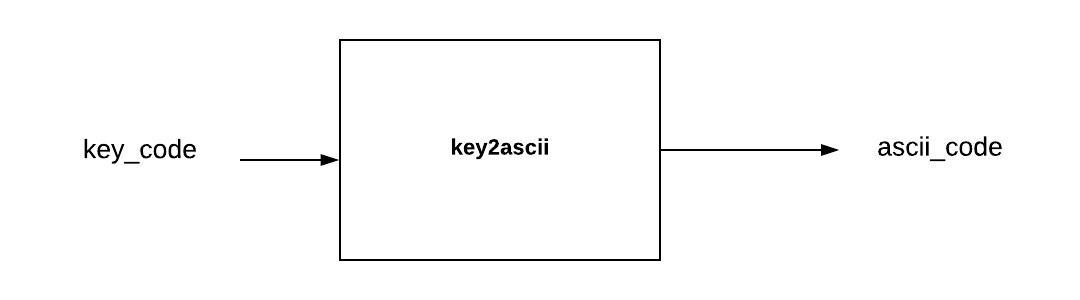
\includegraphics[scale=0.6]{key2ascii.jpeg}
\caption{Módulo key2ascii}
\label{fig:key2ascii}
\end{figure}



\begin{lstlisting}
-- Listing 8.4
library ieee;
use ieee.std_logic_1164.all;
use ieee.numeric_std.all;
entity key2ascii is
   port (
      key_code: in std_logic_vector(7 downto 0);
      ascii_code: out std_logic_vector(7 downto 0)
   );
end key2ascii;

architecture arch of key2ascii is
begin
   with key_code select
      ascii_code <=
         "00110000" when "01000101",  -- 0
         "00110001" when "00010110",  -- 1
         "00110010" when "00011110",  -- 2
         "00110011" when "00100110",  -- 3
         "00110100" when "00100101",  -- 4
         "00110101" when "00101110",  -- 5
         "00110110" when "00110110",  -- 6
         "00110111" when "00111101",  -- 7
         "00111000" when "00111110",  -- 8
         "00111001" when "01000110",  -- 9

         "01000001" when "00011100",  -- A
         "01000010" when "00110010",  -- B
         "01000011" when "00100001",  -- C
         "01000100" when "00100011",  -- D
         "01000101" when "00100100",  -- E
         "01000110" when "00101011",  -- F
         "01000111" when "00110100",  -- G
         "01001000" when "00110011",  -- H
         "01001001" when "01000011",  -- I
         "01001010" when "00111011",  -- J
         "01001011" when "01000010",  -- K
         "01001100" when "01001011",  -- L
         "01001101" when "00111010",  -- M
         "01001110" when "00110001",  -- N
         "01001111" when "01000100",  -- O
         "01010000" when "01001101",  -- P
         "01010001" when "00010101",  -- Q
         "01010010" when "00101101",  -- R
         "01010011" when "00011011",  -- S
         "01010100" when "00101100",  -- T
         "01010101" when "00111100",  -- U
         "01010110" when "00101010",  -- V
         "01010111" when "00011101",  -- W
         "01011000" when "00100010",  -- X
         "01011001" when "00110101",  -- Y
         "01011010" when "00011010",  -- Z

         "01100000" when "00001110",  -- `
         "00101101" when "01001110",  -- -
         "00111101" when "01010101",  -- =
         "01011011" when "01010100",  -- [
         "01011101" when "01011011",  -- ]
         "01011100" when "01011101",  -- \
         "00111011" when "01001100",  -- ;
         "00100111" when "01010010",  -- '
         "00101100" when "01000001",  -- ,
         "00101110" when "01001001",  -- .
         "00101111" when "01001010",  -- /

         "00100000" when "00101001",  -- (space)
         "00001101" when "01011010",  -- (enter, cr)
         "00001000" when "01100110",  -- (backspace)
         "00101010" when others;      -- *
end arch;

} \end{lstlisting}

%%%%%%%%%%%%%%%%% lcd.vhd
\subsection{LCD}

Este foi o único código modificado. O módulo lcd.vhd é responsável pela comunicação com o display LCD da placa FPGA e além disso, toda a lógica da forca juntamente com as chamadas das funções ocorreu nesse arquivo.
A comunicação com o display LCD ocorre através de uma máquina de estados que controla um ponteiro que percorre sequencialmente as posições da tela exibindo no visor o seu valor salvo.
\newline
\begin{figure}[H]
\centering
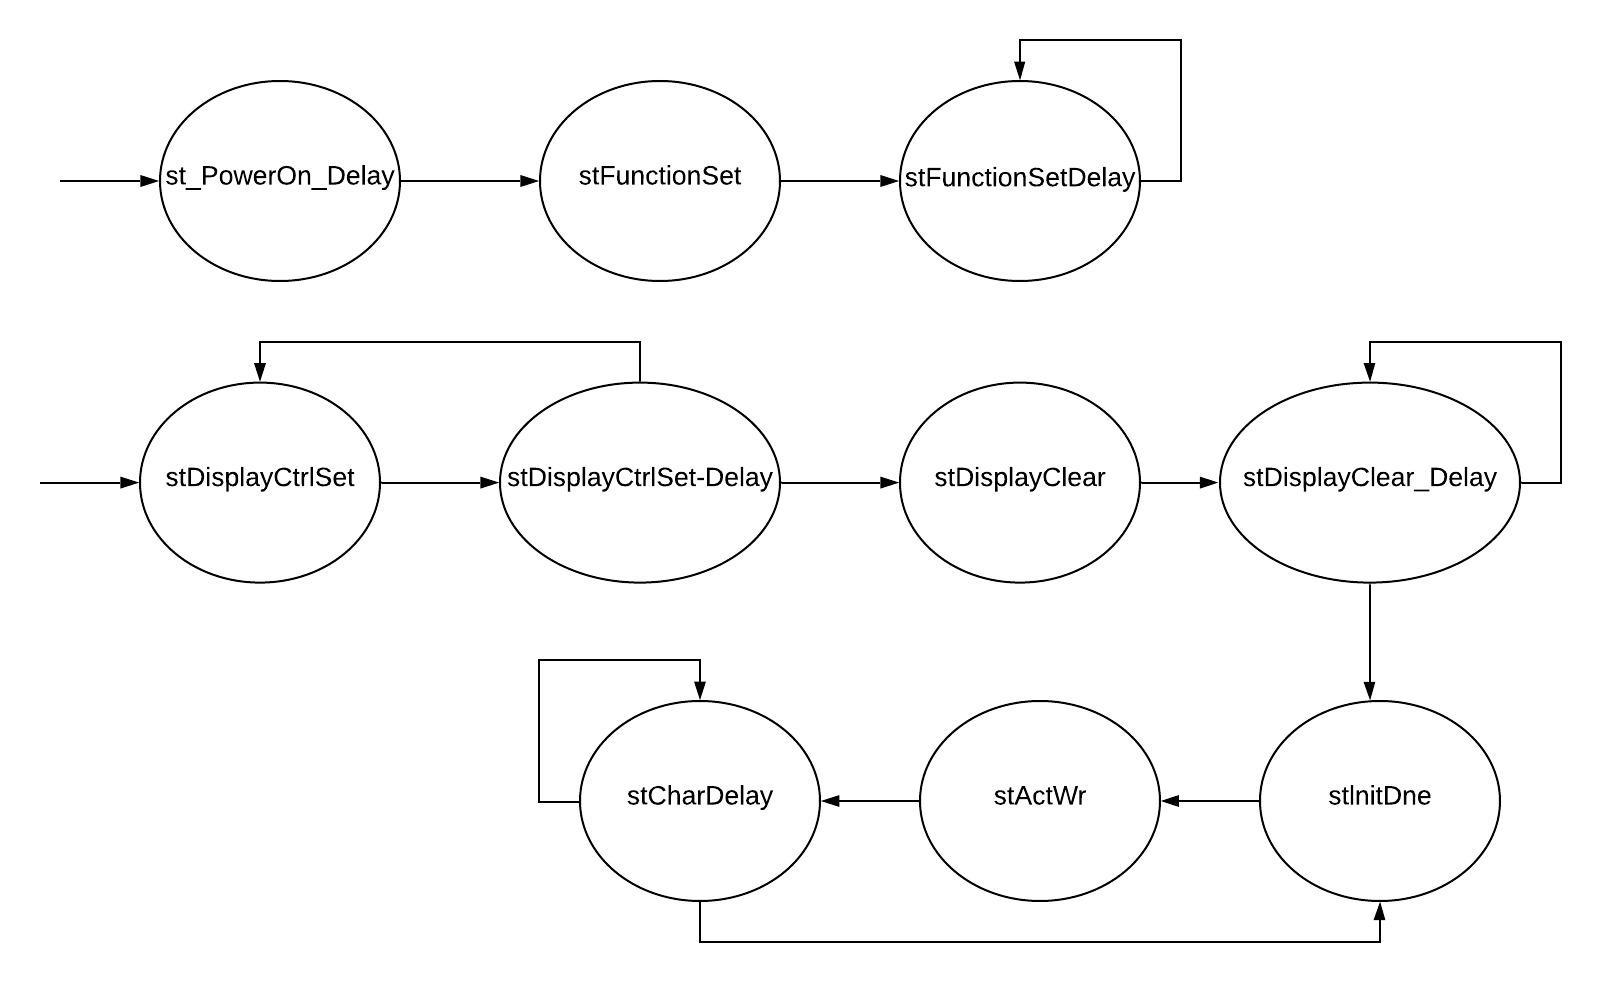
\includegraphics[scale=0.7]{lcd.jpeg}
\caption{Diagrama de estados de lcd.vhd}
\label{fig:lcd}
\end{figure}


Para o funcionamento do jogo, foram utilizados os seguintes sinais e variáveis:\newline
 \begin{itemize}
   \item start : indica o início da "partida" 
   \item vidas : indica o número de vidas restante
   \item palavra\_certa : vetor de 4 bits com o seguinte funcionamento
                    \begin{itemize}
                    \item bit 3 - recebe '1' se bit2 = bit1 = bit0 = '1' (indica que a palavra foi acertada)
                    \item bit 2 - recebe '1' se o usuário digitar a letra D
                    \item bit 1 - recebe '1' se o usuário digitar a letra I
                    \item bit 0 - recebe '1' se o usuário digitar a letra O
                    \end{itemize}
 \end{itemize}

A lógica utilizada está melhor explicada na seção "Funcionamento".



 

\begin{lstlisting}
library IEEE;
use IEEE.STD_LOGIC_1164.ALL;
use IEEE.STD_LOGIC_ARITH.ALL;
use IEEE.STD_LOGIC_UNSIGNED.ALL;



entity lcd is
    Port (
       --- inclusao para kb_code
       ps2d, ps2c: in  std_logic;
       --- 
       LCD_DB: out std_logic_vector(7 downto 0);		
       --DB( 7 through 0)
       RS:out std_logic;                --WE
       RW:out std_logic;                --ADR(0)
       CLK:in std_logic;                --GCLK2
       --ADR1:out std_logic;            --ADR(1)
       --ADR2:out std_logic;            --ADR(2)
       --CS:out std_logic;              --CSC
       OE:out std_logic;                --OE
       KBE:out std_logic;               -- kb_buf_empty
       LEDS: out std_logic_vector(7 downto 0); -- key_code para os LEDs
       rst:in std_logic		);		--BTN
       --rdone: out std_logic);     --WriteDone output to work with DI05 test
end lcd;

architecture Behavioral of lcd is
			    
------------------------------------------------------------------
--  Component Declarations
------------------------------------------------------------------

----INCLUSAO DA FUNCAO KB_CODE PARA LER O TECLADO
component kb_code is
   generic(W_SIZE: integer:=2);  -- 2^W_SIZE words in FIFO
   port (
      clk, reset: in  std_logic;
      ps2d, ps2c: in  std_logic;
      rd_key_code: in std_logic;
      key_code: out std_logic_vector(7 downto 0);
      kb_buf_empty: out std_logic
   );
end component kb_code;

----INCLUSAO DA FUNCAO KEY_2_ASCII PARA CONVERTER AS TECLAS PARA O CODIGO ASCII
component key2ascii is
   port (
      key_code: in std_logic_vector(7 downto 0);
      ascii_code: out std_logic_vector(7 downto 0)
   );
end component key2ascii;

------------------------------------------------------------------
--  Local Type Declarations
-----------------------------------------------------------------
--  Symbolic names for all possible states of the state machines.

	--LCD control state machine
	type mstate is (					  
		stFunctionSet,		 	--Initialization states
		stDisplayCtrlSet,
		stDisplayClear,
		stPowerOn_Delay,  		--Delay states
		stFunctionSet_Delay,
		stDisplayCtrlSet_Delay, 	
		stDisplayClear_Delay,
		stInitDne,			--Display charachters and perform standard operations
		stActWr,
		stCharDelay		--Write delay for operations
		--stWait			--Idle state
	);

	--Write control state machine
	type wstate is (
		stRW,			--set up RS and RW
		stEnable,		--set up E
		stIdle			--Write data on DB(0)-DB(7)
	);

------------------------------------------------------------------
--  Signal Declarations and Constants

    signal clkCount:std_logic_vector(5 downto 0);
    signal activateW:std_logic:= '0';		    			--Activate Write sequence
    signal count:std_logic_vector (16 downto 0):= "00000000000000000";	--15 bit count variable for timing delays
    signal delayOK:std_logic:= '0';						--High when count has reached the right delay time
    signal OneUSClk:std_logic;						--Signal is treated as a 1 MHz clock	
    signal stCur:mstate:= stPowerOn_Delay;					--LCD control state machine
    signal stNext:mstate;			  	
    signal stCurW:wstate:= stIdle; 						--Write control state machine
    signal stNextW:wstate;
    signal writeDone:std_logic;					--Command set finish
    ------- signals para kb_code
    signal rd_key_code: std_logic:= '0';
    signal key_code: std_logic_vector(7 downto 0);
    signal kb_buf_empty: std_logic;
	------- signals para key2ascii
    signal tecla : std_logic_vector(7 downto 0); --ascii_code
	
	-------- signals para logica do jogo
    signal start: std_logic;
    signal palavra_certa : std_logic_vector (3 downto 0) := "0000";
	-- bit 3 - indica se a palavra inteira está certa
	-- bit 2 - indica se a letra D foi encontrada
	-- bit 1 - indica se a letra I foi encontrada
	-- bit 0 - indica se a letra O doi encontrada
	--- >>> Palavra escolhida : DIODO
	
						 
    type LCD_CMDS_T is array(integer range 0 to 30) of std_logic_vector(9 downto 0);
    signal LCD_CMDS : LCD_CMDS_T := ( 
                        0 => "00"&X"3C",            --Function Set
                        1 => "00"&X"0C",			--Display ON, Cursor OFF, Blink OFF
                        2 => "00"&X"01",			--Clear Display
                        3 => "00"&X"02", 		--return home
                        4 => "10"&X"4A", 		-- J
                        5 => "10"&X"6F",  		-- o
                        6 => "10"&X"67",  		-- g
                        7 => "10"&X"6f", 		-- o
                        8 => "10"&X"20", 		-- 
                        9 => "10"&X"64",  		-- d
                        10 => "10"&X"61", 		-- a
                        11 => "10"&X"20", 		--
                        12 => "10"&X"46", 		-- F
                        13 => "10"&X"6f", 		-- o		
                        14 => "10"&X"72",		-- r
                        15 => "10"&X"63", 		-- c
                        16 => "10"&X"61", 		-- a
                        17 => "10"&X"20",		-- 
                        18 => "00"&X"C0",		-- 
                        19 => "10"&X"74",		-- t 
                        20 => "10"&X"65",		-- e
                        21 => "10"&X"63",		-- c
                        22 => "10"&X"6c",		-- l
                        23 => "10"&X"65",		-- e
                        24 => "10"&X"20",		-- 
                        25 => "10"&X"61",		-- a
                        26 => "10"&X"6c",		-- l
                        27 => "10"&X"67",		-- g
                        28 => "10"&X"6f",		-- o
                        29 => "10"&X"20",		-- 
                        30 => "00"&X"02");		-- return home

													
    signal lcd_cmd_ptr : integer range 0 to LCD_CMDS'HIGH + 1 := 0;
begin
	
	--- LEITURA DO TECLADO
    label0 : kb_code port map(CLK,rst,ps2d,ps2c,rd_key_code,key_code,kb_buf_empty);
	--label0 : kb_code port map(CLK,rst,ps2d,ps2c,rd_key_code,key_code,kb_buf_empty);
    KBE <= kb_buf_empty;
    LEDS <= key_code;
	
	--- CONVERSAO PARA ASCII
    label1 : key2ascii port map (key_code , tecla);
	
	

	--  This process counts to 50, and then resets.  It is used to divide the clock signal time.
    process (CLK, oneUSClk)
        begin
            if (CLK = '1' and CLK'event) then
				clkCount <= clkCount + 1;
            end if;
        end process;
	--  This makes oneUSClock peak once every 1 microsecond

    oneUSClk <= clkCount(5);
	--  This process incriments the count variable unless delayOK = 1.
    process (oneUSClk, delayOK)
        begin
            if (oneUSClk = '1' and oneUSClk'event) then
                if delayOK = '1' then
                    count <= "00000000000000000";
                else
                    count <= count + 1;
                end if;
            end if;
    end process;

    --This goes high when all commands have been run
    writeDone <= '1' when (lcd_cmd_ptr = LCD_CMDS'HIGH) 
        else '0';
	--rdone <= '1' when stCur = stWait else '0';
	--Increments the pointer so the statemachine goes through the commands
    process (lcd_cmd_ptr, oneUSClk)
    begin
	
        if (oneUSClk = '1' and oneUSClk'event) then
            if ((stNext = stInitDne or stNext = stDisplayCtrlSet or stNext = stDisplayClear) and writeDone = '0') then 
                lcd_cmd_ptr <= lcd_cmd_ptr + 1;
            elsif stCur = stPowerOn_Delay or stNext = stPowerOn_Delay then
                lcd_cmd_ptr <= 0;
                ------------------------------------------	
            elsif lcd_cmd_ptr = 30 then
                lcd_cmd_ptr <= 3;
                ------------------------------------------
            else
                lcd_cmd_ptr <= lcd_cmd_ptr;
            end if;
        end if;
    end process;
	
	--  Determines when count has gotten to the right number, depending on the state.

    delayOK <= '1' when ((stCur = stPowerOn_Delay and count = "00100111001010010") or 			--20050  
                    (stCur = stFunctionSet_Delay and count = "00000000000110010") or	--50
                    (stCur = stDisplayCtrlSet_Delay and count = "00000000000000010") or	--50
                    --(stCur = stDisplayCtrlSet_Delay and count = "00000000000110010") or	--50
                    (stCur = stDisplayClear_Delay and count = "00000011001000000") or	--1600
                    (stCur = stCharDelay and count = "11111111111111111"))			--Max Delay for character writes and shifts
                    --(stCur = stCharDelay and count = "00000000000100101"))		--37  This is proper delay between writes to ram.
		else	'0';
  	
	-- This process runs the LCD status state machine
	process (oneUSClk, rst)
		begin
			if oneUSClk = '1' and oneUSClk'Event then
				if rst = '1' then
					stCur <= stPowerOn_Delay;
				else
					stCur <= stNext;
				end if;
			end if;
		end process;

	
	--  This process generates the sequence of outputs needed to initialize and write to the LCD screen
    process (stCur, delayOK, writeDone, lcd_cmd_ptr)
        begin   
		
            case stCur is
			
                --  Delays the state machine for 20ms which is needed for proper startup.
				when stPowerOn_Delay =>
                    if delayOK = '1' then
                        stNext <= stFunctionSet;
                    else
                        stNext <= stPowerOn_Delay;
                    end if;
                    RS <= LCD_CMDS(lcd_cmd_ptr)(9);
                    RW <= LCD_CMDS(lcd_cmd_ptr)(8);
                    LCD_DB <= LCD_CMDS(lcd_cmd_ptr)(7 downto 0);
                    activateW <= '0';

                -- This issuse the function set to the LCD as follows 
                -- 8 bit data length, 2 lines, font is 5x8.
                when stFunctionSet =>
                    RS <= LCD_CMDS(lcd_cmd_ptr)(9);
                    RW <= LCD_CMDS(lcd_cmd_ptr)(8);
                    LCD_DB <= LCD_CMDS(lcd_cmd_ptr)(7 downto 0);
                    activateW <= '1';	
                    stNext <= stFunctionSet_Delay;
				
                --Gives the proper delay of 37us between the function set and
                --the display control set.
                when stFunctionSet_Delay =>
                    RS <= LCD_CMDS(lcd_cmd_ptr)(9);
                    RW <= LCD_CMDS(lcd_cmd_ptr)(8);
                    LCD_DB <= LCD_CMDS(lcd_cmd_ptr)(7 downto 0);
                    activateW <= '0';
                    if delayOK = '1' then
                        stNext <= stDisplayCtrlSet;
                    else
                        stNext <= stFunctionSet_Delay;
                    end if;
				
                --Issuse the display control set as follows
                --Display ON,  Cursor OFF, Blinking Cursor OFF.
                when stDisplayCtrlSet =>
                    RS <= LCD_CMDS(lcd_cmd_ptr)(9);
                    RW <= LCD_CMDS(lcd_cmd_ptr)(8);
                    LCD_DB <= LCD_CMDS(lcd_cmd_ptr)(7 downto 0);
                    activateW <= '1';
                    stNext <= stDisplayCtrlSet_Delay;

                --Gives the proper delay of 37us between the display control set
                --and the Display Clear command. 
                when stDisplayCtrlSet_Delay =>
                    RS <= LCD_CMDS(lcd_cmd_ptr)(9);
                    RW <= LCD_CMDS(lcd_cmd_ptr)(8);
                    LCD_DB <= LCD_CMDS(lcd_cmd_ptr)(7 downto 0);
                    activateW <= '0';
                    if delayOK = '1' then
                        stNext <= stDisplayClear;
                    else
                        stNext <= stDisplayCtrlSet_Delay;
                    end if;
				
                --Issues the display clear command.
                when stDisplayClear	=>
                    RS <= LCD_CMDS(lcd_cmd_ptr)(9);
                    RW <= LCD_CMDS(lcd_cmd_ptr)(8);
                    LCD_DB <= LCD_CMDS(lcd_cmd_ptr)(7 downto 0);
                    activateW <= '1';
                    stNext <= stDisplayClear_Delay;

                --Gives the proper delay of 1.52ms between the clear command
                --and the state where you are clear to do normal operations.
                when stDisplayClear_Delay =>
                    RS <= LCD_CMDS(lcd_cmd_ptr)(9);
                    RW <= LCD_CMDS(lcd_cmd_ptr)(8);
                    LCD_DB <= LCD_CMDS(lcd_cmd_ptr)(7 downto 0);
                    activateW <= '0';
                    if delayOK = '1' then
                        stNext <= stInitDne;
                    else
                        stNext <= stDisplayClear_Delay;
                    end if;
				
                --State for normal operations for displaying characters, changing the
                --Cursor position etc.
                when stInitDne =>		
                    RS <= LCD_CMDS(lcd_cmd_ptr)(9);
                    RW <= LCD_CMDS(lcd_cmd_ptr)(8);
                    LCD_DB <= LCD_CMDS(lcd_cmd_ptr)(7 downto 0);
                    activateW <= '0';
                    stNext <= stActWr;

                when stActWr =>		
                    RS <= LCD_CMDS(lcd_cmd_ptr)(9);
                    RW <= LCD_CMDS(lcd_cmd_ptr)(8);
                    LCD_DB <= LCD_CMDS(lcd_cmd_ptr)(7 downto 0);
                    activateW <= '1';
                    stNext <= stCharDelay;
					
                --Provides a max delay between instructions.
                when stCharDelay =>
                    RS <= LCD_CMDS(lcd_cmd_ptr)(9);
                    RW <= LCD_CMDS(lcd_cmd_ptr)(8);
                    LCD_DB <= LCD_CMDS(lcd_cmd_ptr)(7 downto 0);
                    activateW <= '0';					
                    if delayOK = '1' then
                        stNext <= stInitDne;
                    else
                        stNext <= stCharDelay;
                    end if;
            end case;
		
        end process;					
								   
 	--This process runs the write state machine
	process (oneUSClk, rst)
		begin
			if oneUSClk = '1' and oneUSClk'Event then
				if rst = '1' then
					stCurW <= stIdle;
				else
					stCurW <= stNextW;
				end if;
			end if;
		end process;

	--This genearates the sequence of outputs needed to write to the LCD screen
    process (stCurW, activateW)
        begin   
		
            case stCurW is
                --This sends the address across the bus telling the DIO5 that we are
                --writing to the LCD, in this configuration the adr_lcd(2) controls the
                --enable pin on the LCD
                when stRw =>
                    OE <= '0';
                    --CS <= '0';
                    --ADR2 <= '1';
                    --ADR1 <= '0';
                    stNextW <= stEnable;
				
                --This adds another clock onto the wait to make sure data is stable on 
                --the bus before enable goes low.  The lcd has an active falling edge 
                --and will write on the fall of enable
                when stEnable => 
                    OE <= '0';
                    --CS <= '0';
                    --ADR2 <= '0';
                    --ADR1 <= '0';
                    stNextW <= stIdle;
				
                --Waiting for the write command from the instuction state machine
                when stIdle =>
                    --ADR2 <= '0';
                    --ADR1 <= '0';
                    --CS <= '1';
                    OE <= '1';
                    if activateW = '1' then
                        stNextW <= stRw;
                    else
                        stNextW <= stIdle;
                    end if;
                end case;
        end process;
		
	
------ estado para verificar se a letra pertence a palavra ------------------------	
    process(oneUSCLk)
        variable vidas:integer := 5;
    begin
        if (oneUSClk = '1' and oneUSClk'Event) then
			
            if rst = '1' then
                palavra_certa <= "0000";
                vidas := 5;
                start <= '0';
                LCD_CMDS (4) <= "10"&X"4A"; -- J
                LCD_CMDS (5) <= "10"&X"6F"; -- o
                LCD_CMDS (6) <= "10"&X"67"; -- g
                LCD_CMDS (7) <= "10"&X"6F"; -- o
                LCD_CMDS (8) <= "10"&X"20"; --
                LCD_CMDS (9) <= "10"&X"64"; -- d
                LCD_CMDS (10) <= "10"&X"61";-- a
                LCD_CMDS (11) <= "10"&X"20";--
                LCD_CMDS (12) <= "10"&X"46";-- F
                LCD_CMDS (13) <= "10"&X"6f";-- o
                LCD_CMDS (14) <= "10"&X"72";-- r
                LCD_CMDS (15) <= "10"&X"63";-- c
                LCD_CMDS (16) <= "10"&X"61";-- a
                LCD_CMDS (17) <= "10"&X"20";-- 
                LCD_CMDS (18) <= "00"&X"C0";-- 
                LCD_CMDS (19) <= "10"&X"74";-- t 
                LCD_CMDS (20) <= "10"&X"65";-- e
                LCD_CMDS (21) <= "10"&X"63";-- c
                LCD_CMDS (22) <= "10"&X"6c";-- l
                LCD_CMDS (23) <= "10"&X"65";-- e
                LCD_CMDS (24) <= "10"&X"20";-- 
                LCD_CMDS (25) <= "10"&X"61";-- a
                LCD_CMDS (26) <= "10"&X"6c";-- l
                LCD_CMDS (27) <= "10"&X"67";-- g
                LCD_CMDS (28) <= "10"&X"6f";-- o
                LCD_CMDS (29) <= "10"&X"20";-- 	
					
            end if;
			
            if (kb_buf_empty = '1') then
               rd_key_code <= '0';
            end if;
            
			--- mudanca no visor para o inicio do jogo 	
            if (kb_buf_empty = '0') and (start = '0') then
               start <= '1';
               LCD_CMDS (4)  <= "10"&X"5F"; -- _
               LCD_CMDS (5)  <= "10"&X"5F"; -- _
               LCD_CMDS (6)  <= "10"&X"5F"; -- _
               LCD_CMDS (7)  <= "10"&X"5F"; -- _
               LCD_CMDS (8)  <= "10"&X"5F"; -- _
               LCD_CMDS (9)  <= "10"&X"20"; --
               LCD_CMDS (10) <= "10"&X"20"; --
               LCD_CMDS (11) <= "10"&X"20"; --
               LCD_CMDS (12) <= "10"&X"20"; --
               LCD_CMDS (13) <= "10"&X"20"; --
               LCD_CMDS (14) <= "10"&X"20"; --
               LCD_CMDS (15) <= "10"&X"20"; --
               LCD_CMDS (16) <= "10"&X"20"; --
               LCD_CMDS (17) <= "10"&X"35"; -- 5
               LCD_CMDS (18) <= "00"&X"C0"; -- "pular linha" 
               LCD_CMDS (19) <= "10"&X"20"; --  
               LCD_CMDS (20) <= "10"&X"20"; -- 
               LCD_CMDS (21) <= "10"&X"20"; -- 
               LCD_CMDS (22) <= "10"&X"20"; -- 
               LCD_CMDS (23) <= "10"&X"20"; -- 
               LCD_CMDS (24) <= "10"&X"20"; -- 
               LCD_CMDS (25) <= "10"&X"20"; -- 
               LCD_CMDS (26) <= "10"&X"20"; -- 
               LCD_CMDS (27) <= "10"&X"20"; -- 
               LCD_CMDS (28) <= "10"&X"20"; -- 
               LCD_CMDS (29) <= "10"&X"20"; -- 	
               rd_key_code <= '1';
            end if;
			
            --- analise das teclas
            if ((start = '1') and (vidas > 0) and (kb_buf_empty = '0') and (palavra_certa /= "1111")) then 
               
               case tecla is
                   when X"44" => --- verifica se a letra salva foi D
                           if (palavra_certa(2) = '0') then -- D____
                               palavra_certa(2) <= '1';
						end if;
					
                   when X"49" => -- verifica se a letra salva foi I
                           if (palavra_certa(1) = '0') then -- _I___
                               palavra_certa(1) <= '1';
						end if;
					
                   when X"4F" => -- verifica se a letra salva foi O
                           if (palavra_certa(0) = '0') then -- __O__
                               palavra_certa(0) <= '1';
						end if;
                   when others =>
                           vidas := vidas - 1;
					
               end case;		
               rd_key_code <= '1'; 
            end if;
			
			--- palavra encontrada
            if (palavra_certa = "0111") then
               palavra_certa <= "1111";
            end if;
		
--------  trocar "_" pela letra certa (ou manter inalterado)
            if(start = '1') then
               if (palavra_certa(2) = '1') then
                   LCD_CMDS(4) <= "10"&X"44"; -- escreve D
                   LCD_CMDS(7) <= "10"&X"44";
               else 
                   LCD_CMDS(4) <= "10"&X"5F";	
                   LCD_CMDS(7) <= "10"&X"5F";
               end if;
        		
               if (palavra_certa(1) = '1') then
                   LCD_CMDS(5) <= "10"&X"49"; -- escreve I
               else 
                   LCD_CMDS(5) <= "10"&X"5F";
               end if;
        		
               if (palavra_certa(0) = '1') then
                   LCD_CMDS(6) <= "10"&X"4F"; -- escreve O
                   LCD_CMDS(8) <= "10"&X"4F";
               else 
                   LCD_CMDS(6) <= "10"&X"5F"; 
                   LCD_CMDS(8) <= "10"&X"5F";
               end if;
            end if;

		
------- analise das vidas 
            if (vidas /= 5) then
    			case vidas is
    			
                   when 4 => 
                           LCD_CMDS(17) <= "10"&X"34"; -- escreve 4
    	
                   when 3 =>
                           LCD_CMDS(17) <= "10"&X"33"; -- escreve 3
    		
                   when 2 =>
                           LCD_CMDS(17) <= "10"&X"32"; -- escreve 2	
    			
                   when 1 =>
                           LCD_CMDS(17) <= "10"&X"31"; -- escreve 1
    				
                   when others => ------- estado "perdeu"
                           LCD_CMDS(17) <= "10"&X"30"; -- escreve 0
                           LCD_CMDS(4) <= LCD_CMDS(4);  
                           LCD_CMDS(5) <= LCD_CMDS(5);  
                           LCD_CMDS(6) <= LCD_CMDS(6); 	
                           LCD_CMDS(7) <= LCD_CMDS(7);  
                           LCD_CMDS(8) <= LCD_CMDS(8);  
                           LCD_CMDS(9) <= LCD_CMDS(9);  
                           LCD_CMDS(10) <= LCD_CMDS(10);  
                           LCD_CMDS(11) <= LCD_CMDS(11); 
                           LCD_CMDS(12) <= LCD_CMDS(12); 
                           LCD_CMDS(13) <= LCD_CMDS(13); 
                           LCD_CMDS(14) <= LCD_CMDS(14); 
                           LCD_CMDS(15) <= LCD_CMDS(15); 
                           LCD_CMDS(16) <= LCD_CMDS(16); 
                           LCD_CMDS(18) <= "00"&X"C0";-- 
                           LCD_CMDS(19) <= "10"&X"56";-- V
                           LCD_CMDS(20) <= "10"&X"4F";-- O
                           LCD_CMDS(21) <= "10"&X"43";-- C
                           LCD_CMDS(22) <= "10"&X"45";-- E
                           LCD_CMDS(23) <= "10"&X"20";-- 
                           LCD_CMDS(24) <= "10"&X"50";-- P
                           LCD_CMDS(25) <= "10"&X"45";-- E 
                           LCD_CMDS(26) <= "10"&X"52";-- R
                           LCD_CMDS(27) <= "10"&X"44";-- D
                           LCD_CMDS(28) <= "10"&X"45";-- E
                           LCD_CMDS(29) <= "10"&X"55";-- U
    				
                   end case;
            end if;

------ estado "ganhou"  	
            case palavra_certa is
                   when "1111" =>
                           LCD_CMDS(4) <= LCD_CMDS(4);  
                           LCD_CMDS(5) <= LCD_CMDS(5);  
                           LCD_CMDS(6) <= LCD_CMDS(6); 	
                           LCD_CMDS(7) <= LCD_CMDS(7);  
                           LCD_CMDS(8) <= LCD_CMDS(8);  
                           LCD_CMDS(9) <= LCD_CMDS(9);  
                           LCD_CMDS(10) <= LCD_CMDS(10);  
                           LCD_CMDS(11) <= LCD_CMDS(11); 
                           LCD_CMDS(12) <= LCD_CMDS(12); 
                           LCD_CMDS(13) <= LCD_CMDS(13); 
                           LCD_CMDS(14) <= LCD_CMDS(14); 
                           LCD_CMDS(15) <= LCD_CMDS(15); 
                           LCD_CMDS(16) <= LCD_CMDS(16); 
                           LCD_CMDS(17) <= LCD_CMDS(17); 
                           LCD_CMDS(18) <= "00"&X"C0";-- 
                           LCD_CMDS(19) <= "10"&X"56";-- V
                           LCD_CMDS(20) <= "10"&X"4F";-- O
                           LCD_CMDS(21) <= "10"&X"43";-- C
                           LCD_CMDS(22) <= "10"&X"45";-- E
                           LCD_CMDS(23) <= "10"&X"20";-- 
                           LCD_CMDS(24) <= "10"&X"47";-- G
                           LCD_CMDS(25) <= "10"&X"41";-- A 
                           LCD_CMDS(26) <= "10"&X"4E";-- N
                           LCD_CMDS(27) <= "10"&X"48";-- H
                           LCD_CMDS(28) <= "10"&X"4F";-- O
                           LCD_CMDS(29) <= "10"&X"55";-- U
    
    
                   when others =>
            end case;

--------------------
		end if;
	end process;					
end Behavioral;

--------------------
} \end{lstlisting}

\section{Funcionamento}

Para o funcionamento da forca, fizemos uma analogia com uma máquina de estados e desenvolmos o código vhdl para executá-la. A máquina é dividida em 5 estados assim como representado na Figura \ref{fig:diagramajogo}.

%%%%%%%%%%%%%  DIAGRAMA DE ESTADOS 
\begin{figure}[H]
\centering
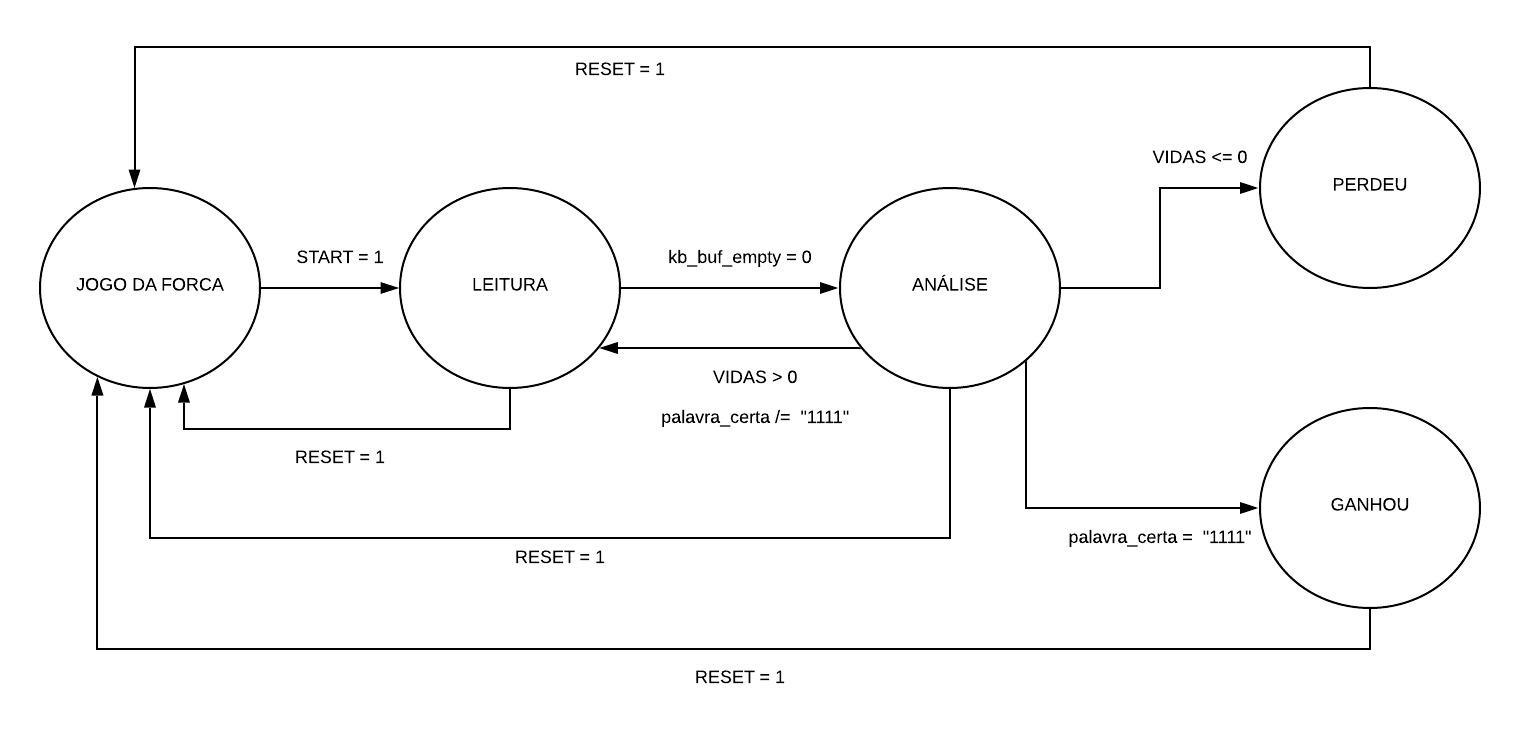
\includegraphics[scale=0.6]{diagramajogo.jpeg}
\caption{Diagrama de estados}
\label{fig:diagramajogo}
\end{figure}

No estado inicial uma frase é mostrada na tela (Figura \ref{fig:telainicial}) e permanece estática aguardando o sinal de start dado pelo jogador e para isso basta que ele aperte qualquer tecla. 
obs.: a tecla pressionada para dar o sinal de start não é salva e não afeta a pontuação do jogo.

\begin{figure}[H]
\centering
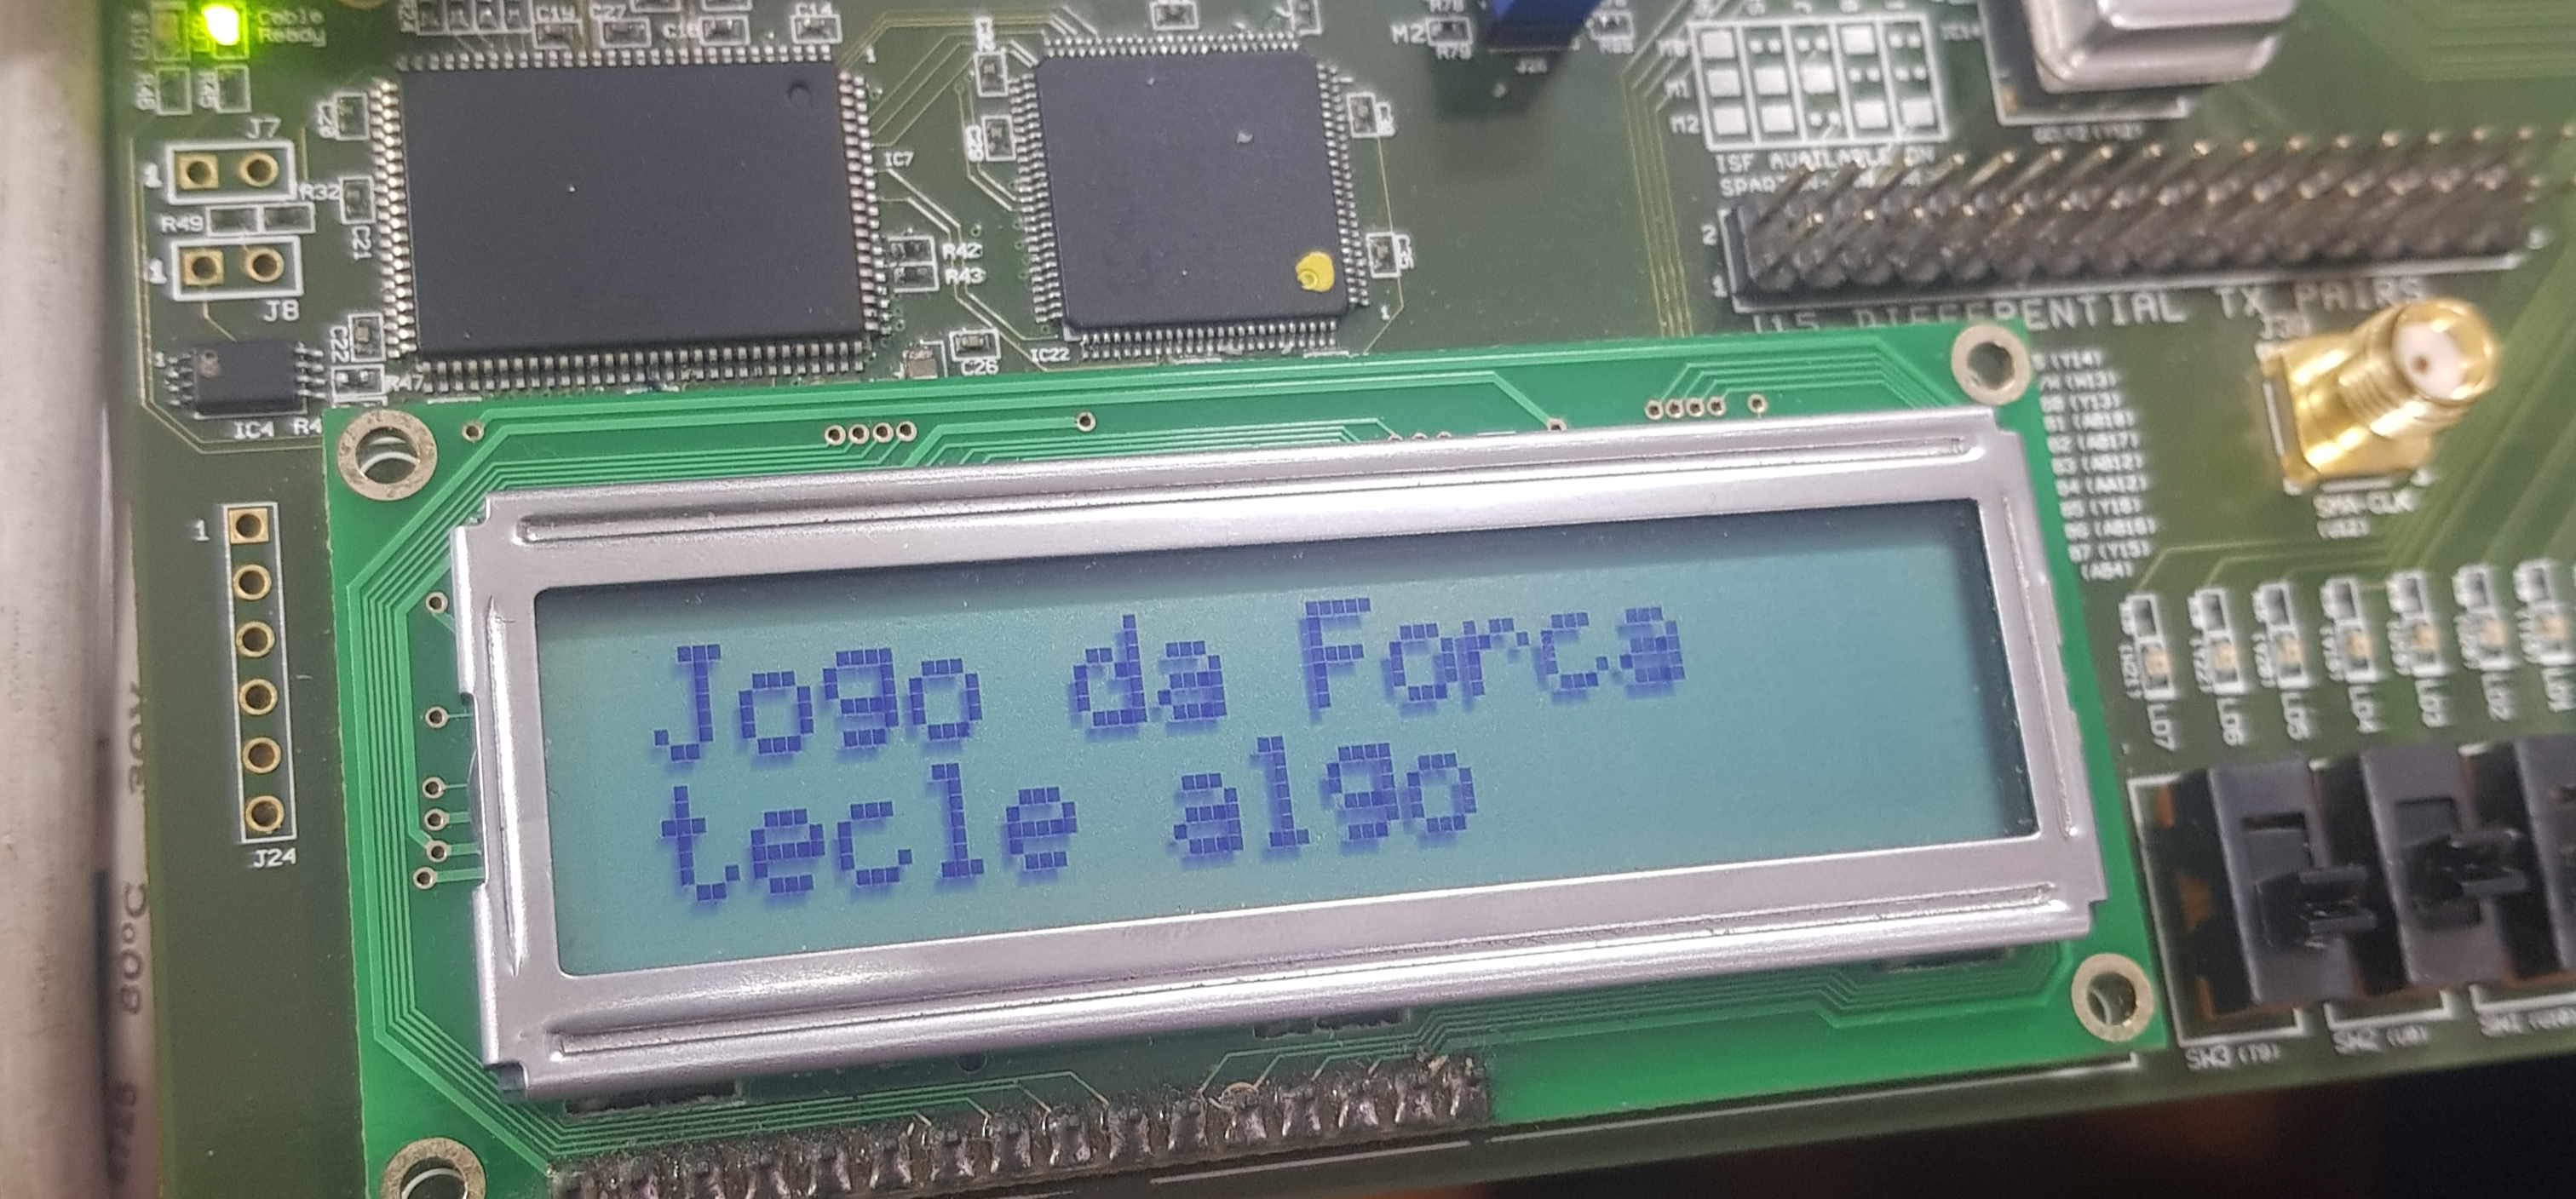
\includegraphics[scale=0.1]{inicio.jpg}
\caption{tela inicial}
\label{fig:telainicial}
\end{figure}

Após o sinal de start, uma nova tela mostra 5 espaços para as 5 letras da palavra além do número de vidas restantes (inicialmente 5). A máquina alterna entre os estados de leitura e análise da letra. No estado de leitura nada acontece até que uma tecla seja pressionada ( kb\_buf\_empty recebe '0'). Quando isso aconte, ela migra para o estado de análise onde a tecla pressionada pelo usuário é salva e analisada. \\
Se a letra salva estiver na palavra, ela é revelada nos 5 espaços inicialmente vazios, se a letra não estiver na palavra, o número de vidas é diminuído em 1 unidade. Se a palavra não for encontrada (palavra\_certa diferente de "1111") e o usuário ainda tiver vidas restantes (vidas $>$ 0), então a máquina retorna para o estado de leitura e realiza esse ciclo novamente. 
\\
Se o usuário completar a palavra antes de perder suas vidas (palavra\_certa = "1111"), a máquina passa para o estado "ganhou" e a frase "Você Ganhou" aparece na tela (Figura \ref{fig:ganhou}) terminando o jogo e deixando a tela estática até um possível sinal de reset.
\begin{figure}[H]
\centering
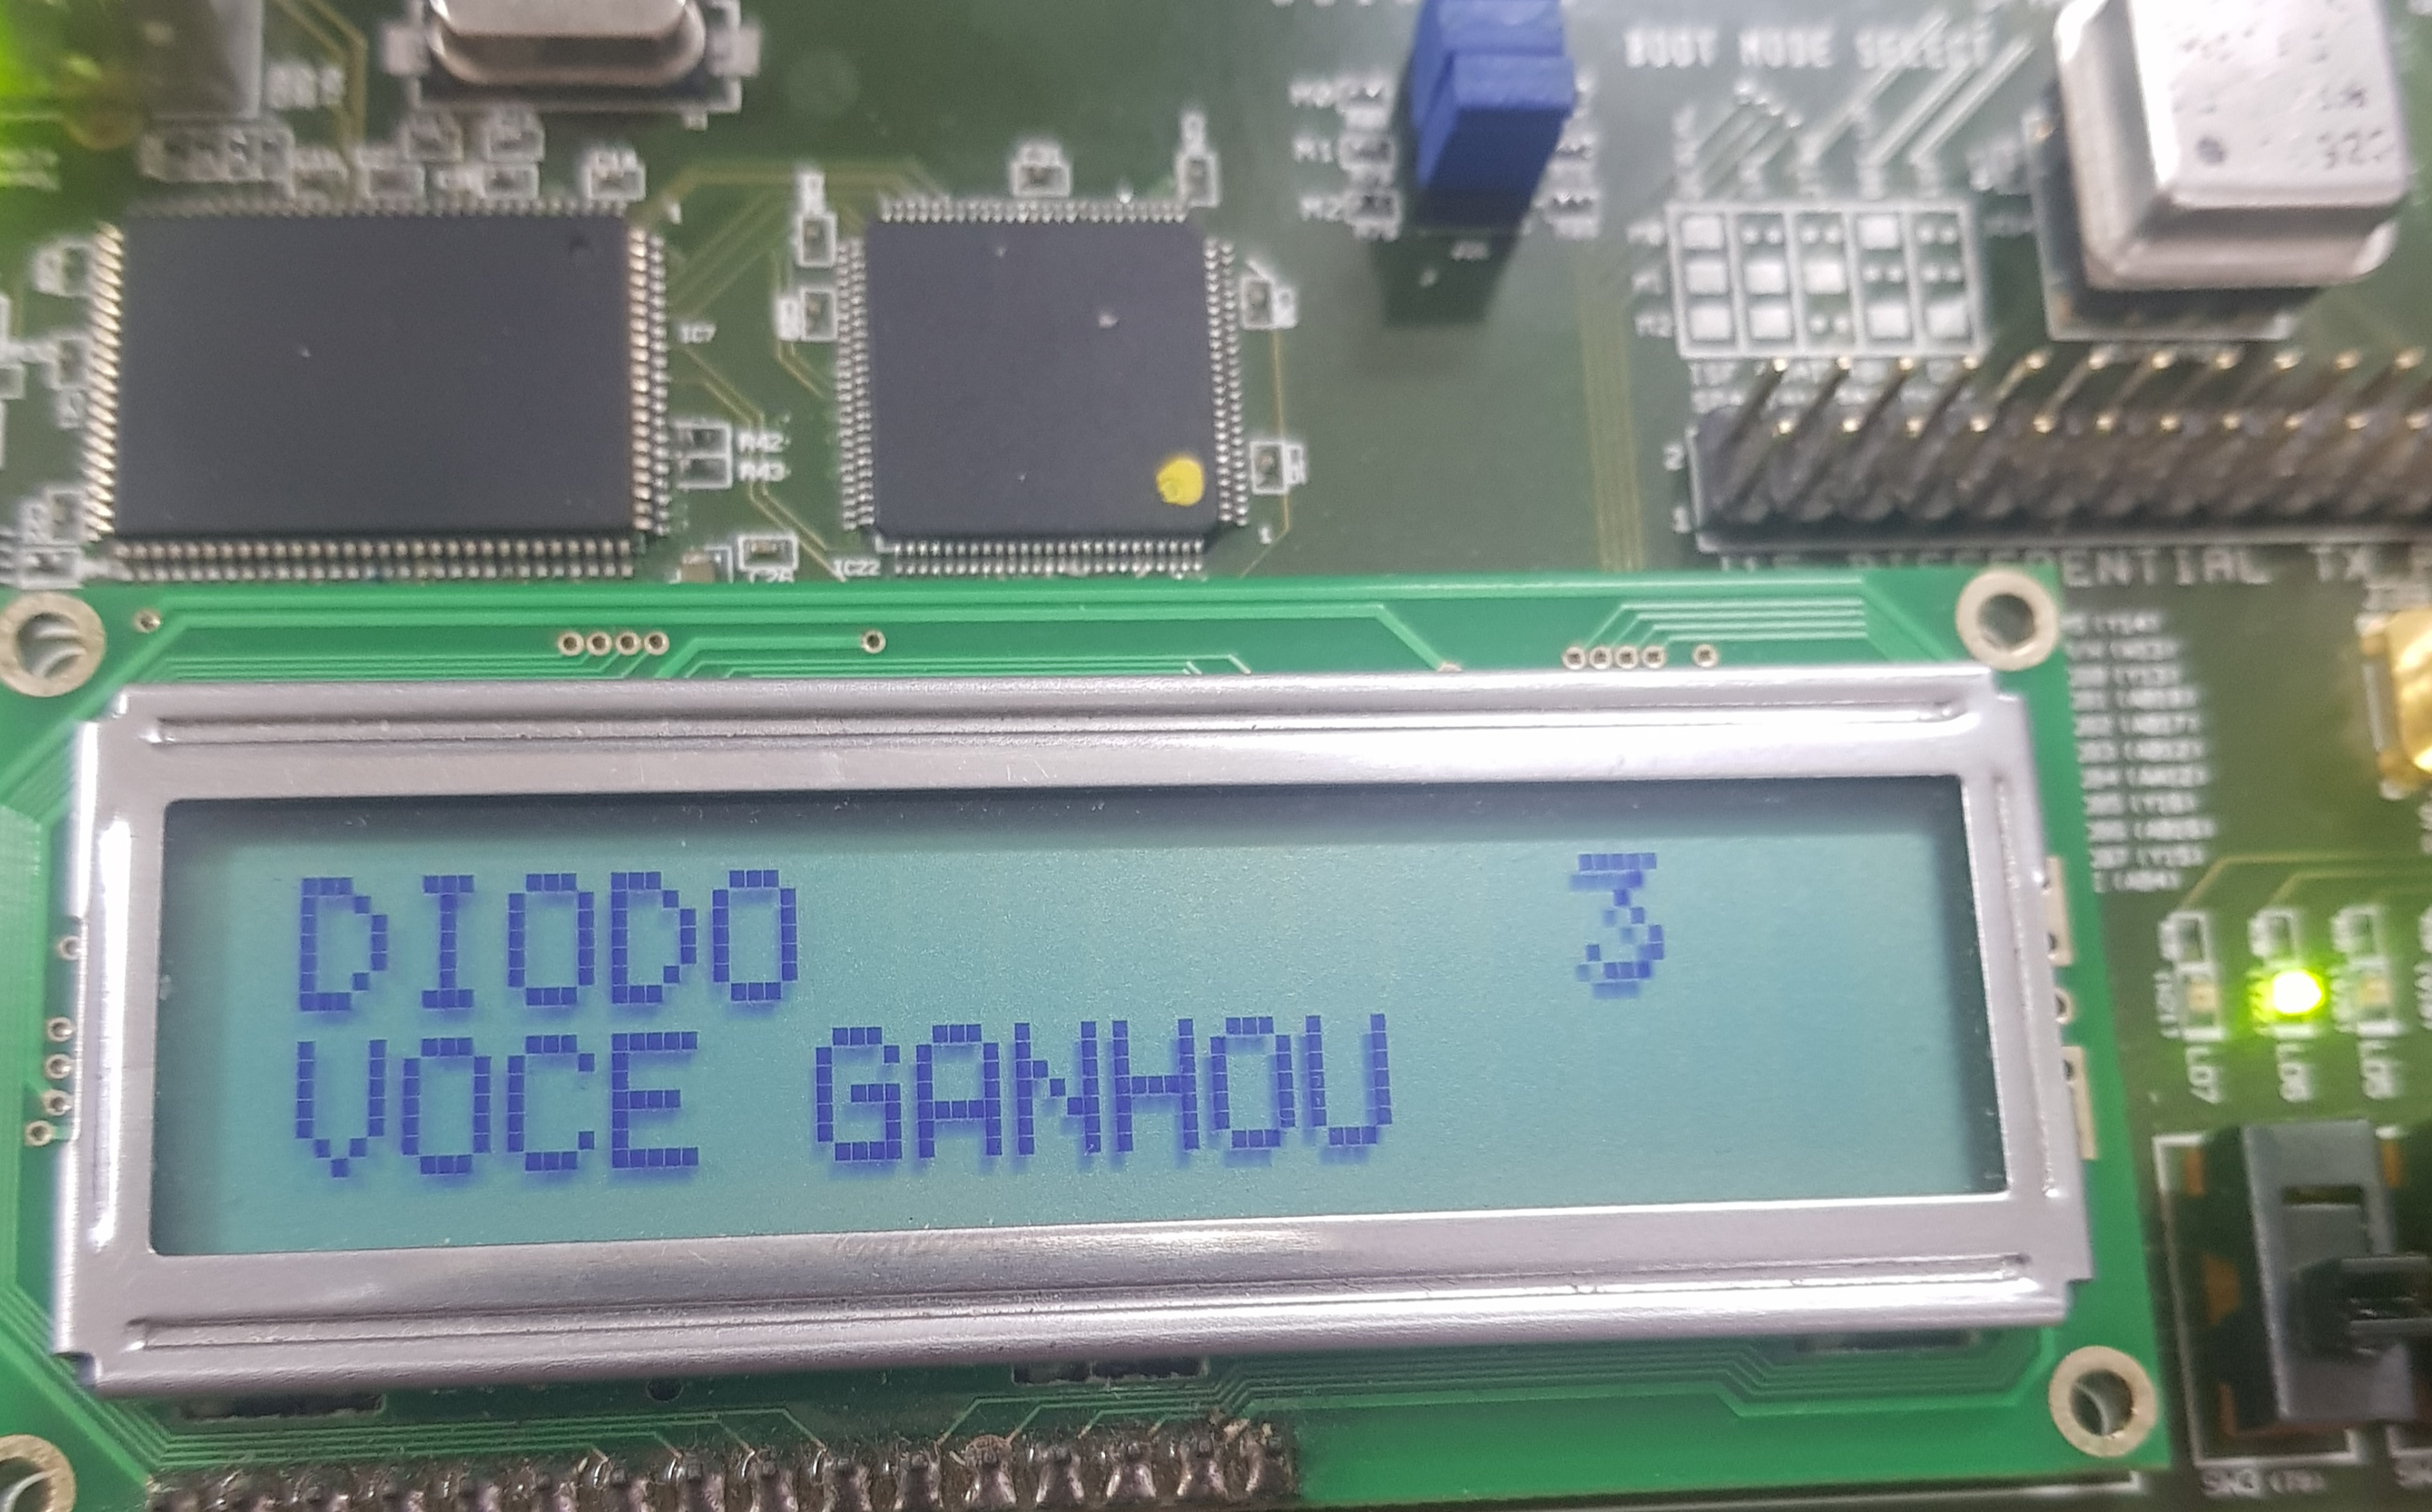
\includegraphics[scale=0.1]{ganhou.jpg}
\caption{tela ao ganhar o jogo}
\label{fig:ganhou}
\end{figure}

 Se o número de vidas chegar a zero antes do usuário completar a palavra (vidas = 0), a máquina passa para o estado "perdeu" e a frase "Você Perdeu" aparece na tela (Figura \ref{fig:perdeu}) terminando o jogo e deixando a tela estática até um possível sinal de reset.
\begin{figure}[H]
\centering
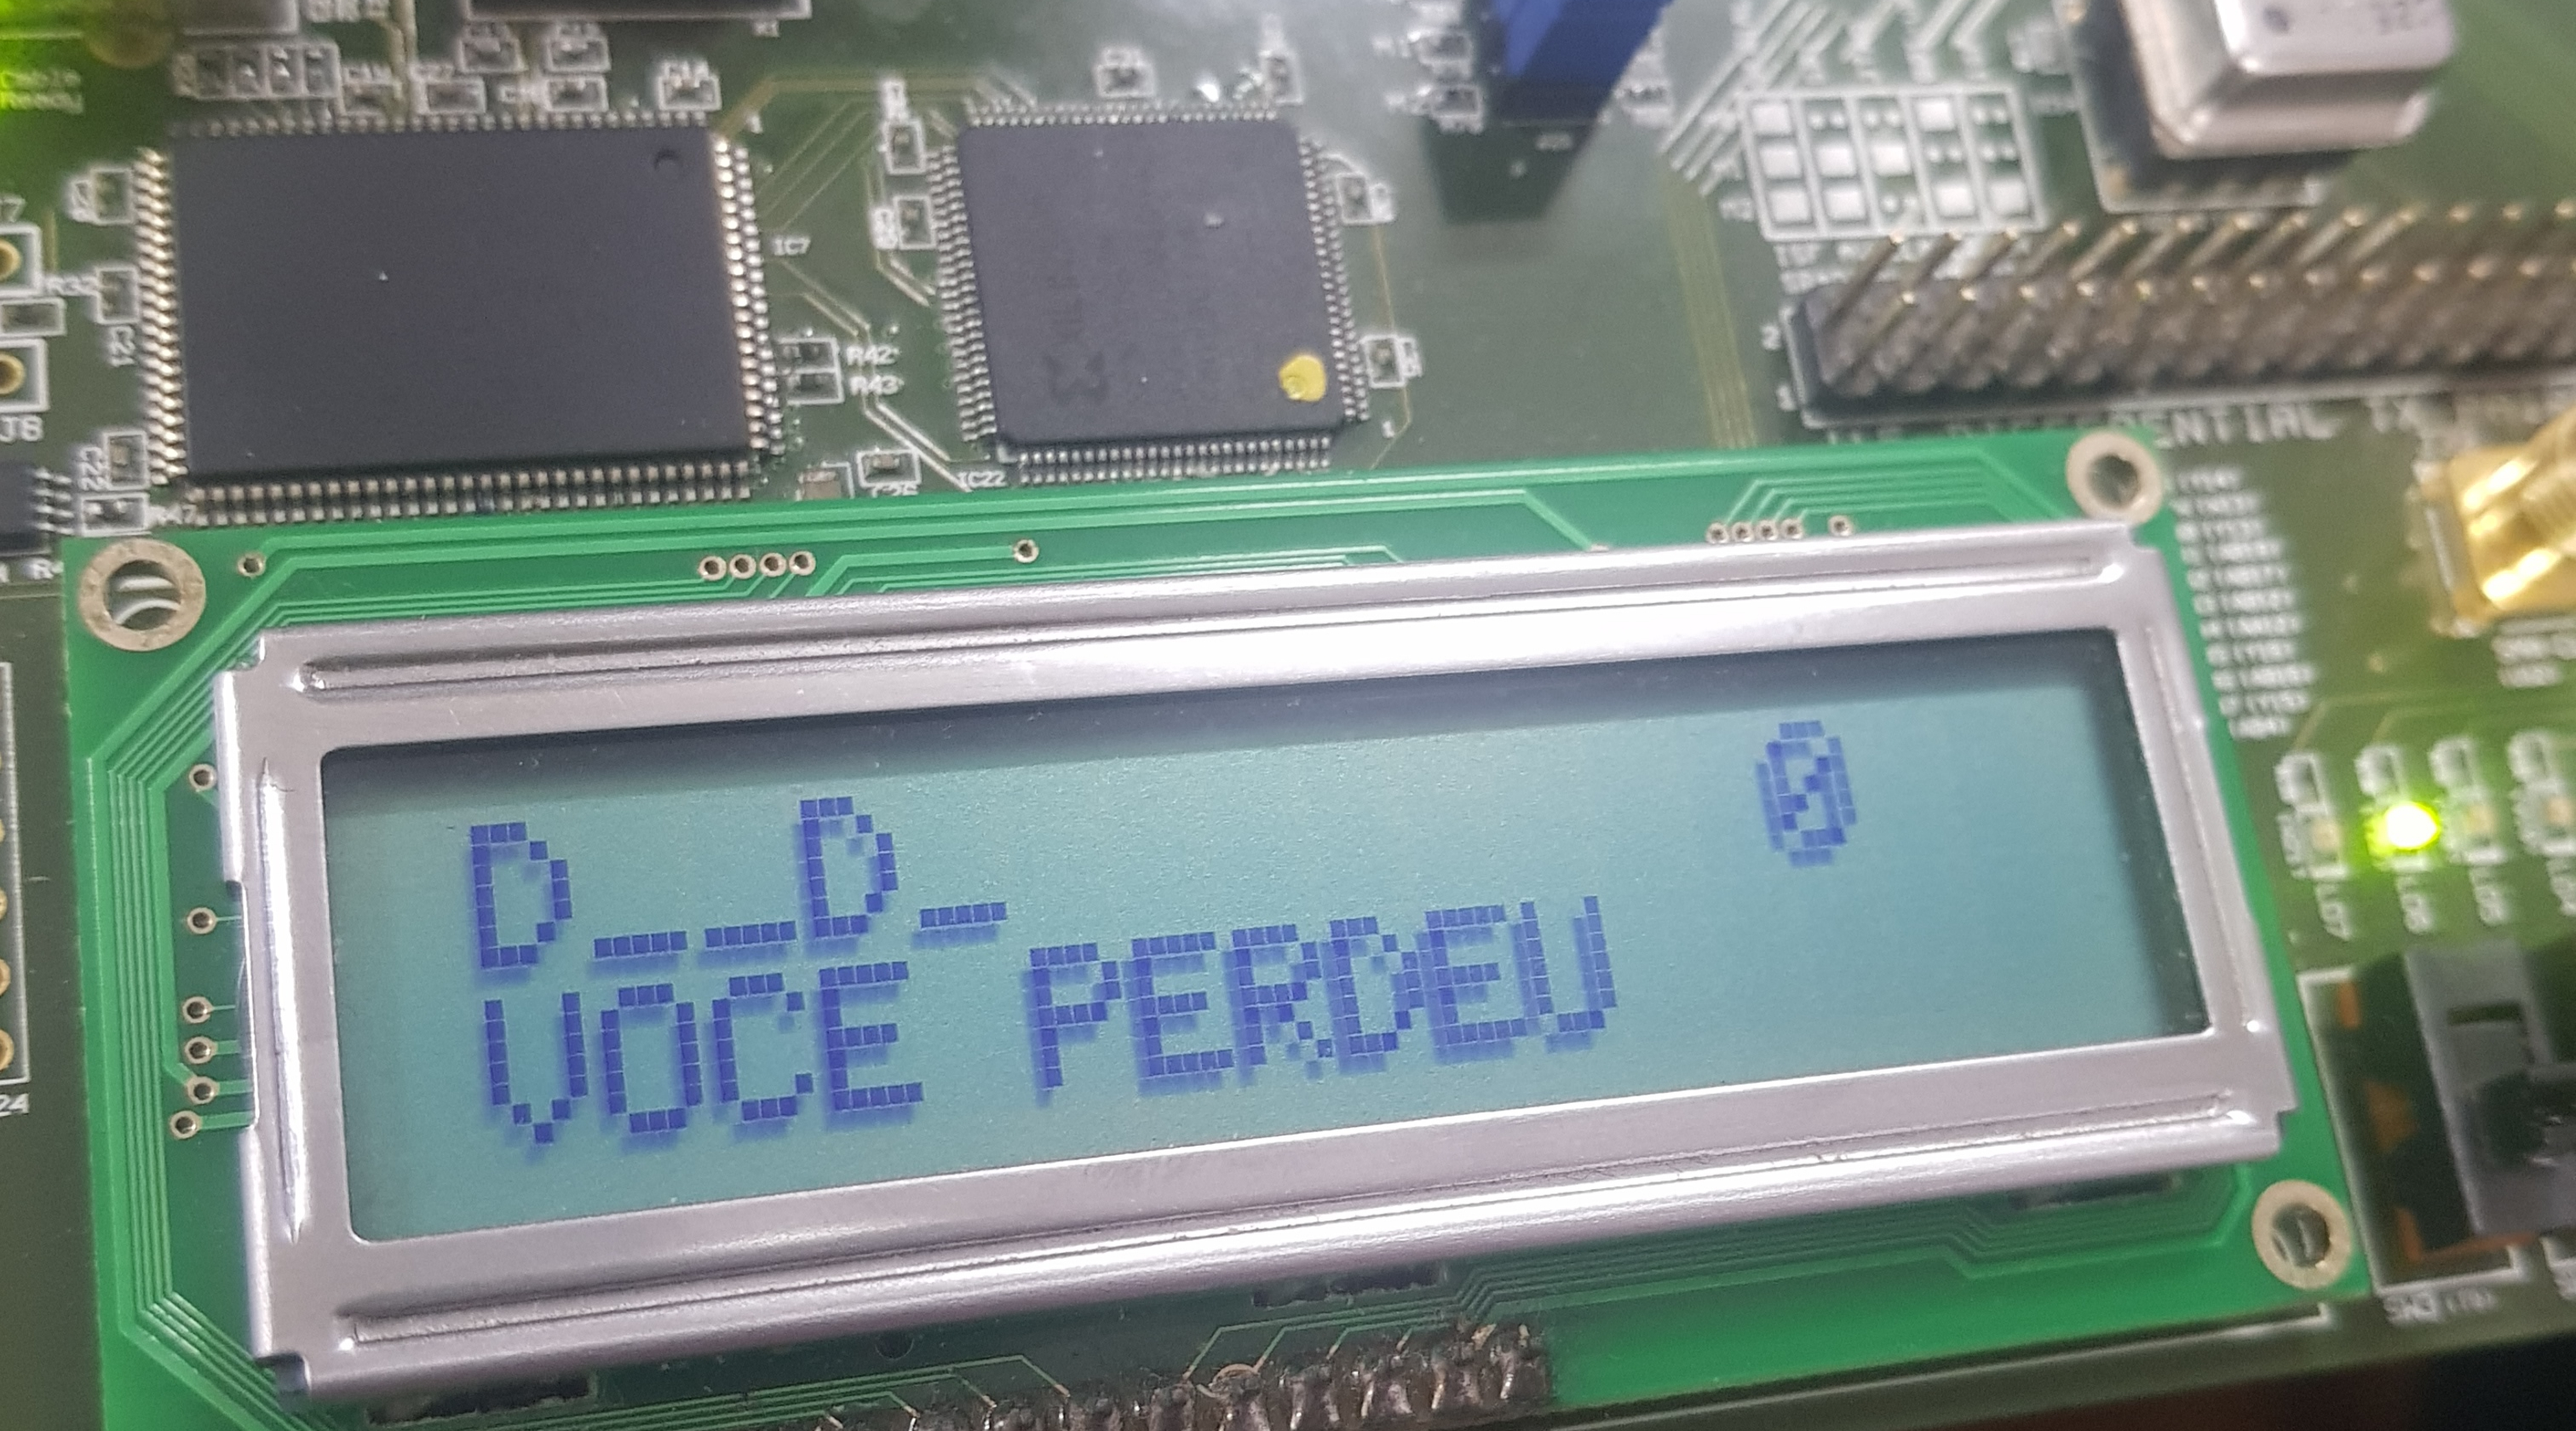
\includegraphics[scale=0.1]{perdeu.jpg}
\caption{tela ao perder o jogo}
\label{fig:perdeu}
\end{figure}

Em  qualquer estado, o sinal de resest ativo (rst = 1) faz o jogo voltar ao estado inicial.

%%%%%%%%%%%%%%%%%%%%%%%%%%%%%%%%%%%%%%%%%%%%%%%%%%%%%%%%%%%%%%%%%%%
\section{Conclusão}
    Após o desenvolvimento dos códigos e dezenas de testes o jogo funcionou corretamente e o projeto foi finalizado como esperado.
%%%%%%%%%%%%%%%%%%%%%%%%%%%%%%%%%%%%%%%%%%%%%%%%%%%%%%%%%%%%%%%%%%%
\section{Bibliografia}
\begin{enumerate}
    \item https://pt.wikipedia.org/wiki/PS/2
    \item https://https://pt.wikipedia.org/wiki/FIFO
   \item https://www.gta.ufrj.br/ensino/EEL480/index.html

 \end{enumerate}



\end{document}
